\documentclass[
  dvipdfmx,
  xcolor={svgnames},
  hyperref={colorlinks,citecolor=DeepPink4,linkcolor=DarkRed,urlcolor=DarkBlue}
  ]{beamer}
\title{}
\title[A proposal of semantic segmentation model for Gleason patterns and integrated diagnostic system using Raspberry Pi]{A proposal for semantic segmentation model for evaluating Gleason patterns of prostate cancer and integrated diagnostic system using Raspberry Pi}
\author{Ken Enda}

\institute{Department of Cancer Pathology Faculty of Medicine, HOKKAIDO UNIVERSITY}

\date[]{June, 2020}

\usetheme{metropolis}
% \usetheme{Berlin}

\usepackage[utf8]{inputenc}
% \usepackage{bxdpx-beamer}
% \usepackage{pxjahyper}
\usepackage{graphicx}
\usepackage{media9}
\usepackage{hyperref}
% \usepackage{movie15}
% \usepackage{parskip}

\newcommand\Fontvi{\fontsize{6}{7.2}\selectfont}

% \usepackage[orientation=portrait,size=a0,scale=1.4,debug]{beamerposter}
\usepackage[japanese]{babel}
\usepackage[font=small]{caption}
\usepackage[font=footnotesize]{subcaption}
\setbeamertemplate{navigation symbols}{}

% caption
\addto\captionsjapanese{\renewcommand{\figurename}{Fig}}
\addto\captionsjapanese{\renewcommand{\tablename}{Table}}
\setbeamertemplate{caption}[numbered]

% bib
\renewcommand{\kanjifamilydefault}{\gtdefault}
\setbeamercolor{bibliography item}{fg=black}
\setbeamercolor{bibliography entry author}{fg=black}
% \setbeamercolor{bibliography entry author}{fg=red}
% \setbeamercolor{bibliography entry title}{fg=blue}
% \setbeamercolor{bibliography entry location}{fg=green}
% \setbeamercolor{bibliography entry note}{fg=cyan}

\setbeamerfont{bibliography item}{size=\scriptsize}
\setbeamerfont{bibliography entry author}{size=\scriptsize}
\setbeamerfont{bibliography entry title}{size=\scriptsize}
\setbeamerfont{bibliography entry location}{size=\scriptsize}
\setbeamerfont{bibliography entry note}{size=\scriptsize}
\addtobeamertemplate{footline}{\hypersetup{allcolors=.}}{}

% fig
\makeatletter
\def\@cite#1{\textsuperscript{[#1]}}
\makeatother

\begin{document}
\nocite{*}

\begin{frame}{}
  \huge A proposal for semantic segmentation model for evaluating Gleason patterns of prostate cancer and integrated diagnostic system using Raspberry Pi\par
  \vspace{0.5zh}
  \normalsize Ken ENDA \cite{student} Koki ISE\cite{student} Yusuke ISHIDA\cite{dept} Sinya TANAKA\cite{dept}\cite{icredd}\cite{gicore}
  \begin{thebibliography}{99}
    \beamertemplatetextbibitems
    \setlength{\itemsep}{-.5zw}
    \bibitem{student} Sch. Med., Hokkaido Univ.
    \bibitem{dept} Dept. Cancer Pathol., Fac. Med., Hokkaido Univ.
    \bibitem{icredd} Inst. Chem. Reaction Design and Discovery (WPI-ICReDD), Hokkaido Univ.  
    \bibitem{gicore} Global Inst. Collaborative Res. Edu. (GI-CoRE), Hokkaido Univ.
  \end{thebibliography}
\end{frame}


\begin{frame}{COI}
    \setlength{\fboxsep}{1em}
    \fbox{
      \parbox{22em}{
        \centering
        \Huge 第109回日本病理学会総会COI開示
        \par
        \vspace{0.5zh}
        \large 筆頭発表者名:遠田 建
      }
    }
    \par
    \vspace{1zh}
  \centering 演題発表に関連し、開示すべきCOI関係にある企業などはありません。
\end{frame}

\begin{frame}{Introduction}
  In recent years, image analysis of histopathology field has been remarkably improved due to deep learning (DL) method using convolutional network. On the other hand, not many facilities are using DL system for its initial cost or unproven reliability. Several steps required to obtain inferential results from DL on histopathological images.
\end{frame}

\begin{frame}{Introduction}
  Now if some pathologists going to harness DL system power for their diagnostic assistant; taking microscopic digital photo-image, choose an image appropriate for diagnosis, transfer the image files to an external or network storage, then start up DL system, read target file, overlaying the original image and DL output file for comparison, finally the pathologist get the reliable output and interpret into the final diagnosis.
\end{frame}

\begin{frame}{Introduction}
  Due to these hassle things, DL are rarely used directly in clinical practice nowadays.
  \par
  \vspace{0.5zh}
  In this study, we integrated the system of microscopic image capture and overlaying DL output image for clinical diagnostics, using a small and very low cost Raspberry Pi computer.
\end{frame}

\begin{frame}{Material and method}
  In our previous study, we have established the U-Net\cite{unet} model of semantic segmentation for detecting prostatic cancers based on Gleason pattern(GP).
  \par
  \vspace{0.5zh}
  Our U-Net model consists of pretrained VGG16\cite{vgg} encoder and nearest sampling decoder\cite{ternausnet}. The training data were the histopathology images of total prostatectomy, labeled by trained pathologists of our laboratory, as normal glands, GP3, GP4, and GP5 (Fig.\ref{fig:seg_color}).
\end{frame}

\begin{frame}{Material and method}

  \begin{figure}[htbp]\centering
    \begin{tabular}{c}
      \begin{subfigure}[t]{0.33\columnwidth}\centering
        
\includegraphics[]{assets/gp_pin.png}
        \subcaption{Normal glands:black}
      \end{subfigure}

      \begin{subfigure}[t]{0.33\columnwidth}\centering
        
\includegraphics[]{assets/gp_3_2.png}
        \subcaption{GP3:blue}
      \end{subfigure}

      \begin{subfigure}[t]{0.33\columnwidth}\centering
        
\includegraphics[]{assets/gp_4.png}
        \subcaption{GP4:green}
      \end{subfigure}
    \end{tabular}

    \begin{tabular}{c}
      \begin{subfigure}[t]{0.33\columnwidth}\centering
        
\includegraphics[]{assets/gp_5_2.png}
        \subcaption{GP5:red}
      \end{subfigure}

      \begin{subfigure}[t]{0.33\columnwidth}\centering
        
\includegraphics[]{assets/gp_3_1.png}
        \subcaption{GP3+4}
      \end{subfigure}

      \begin{subfigure}[t]{0.33\columnwidth}\centering
        
\includegraphics[]{assets/gp_5_1.png}
        \subcaption{GP4+5}
      \end{subfigure}
    \end{tabular}
    \label{fig:example}
    \caption{Example of the segmentation}
    \label{fig:seg_color}
  \end{figure}
\end{frame}

\begin{frame}{Material and method}
  An output example of our model is shown in Fig.2.
  \begin{figure}[htbp]\centering
    \begin{tabular}{c}
      \begin{subfigure}[t]{0.33\columnwidth}\centering
        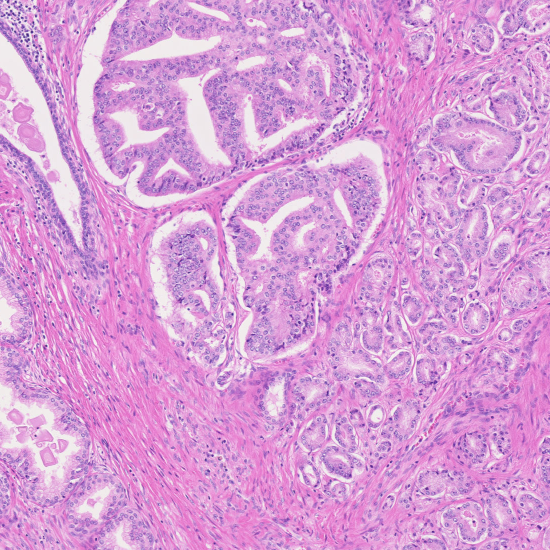
\includegraphics[width=0.9\columnwidth]{assets/ex_org.png}
        \subcaption{Input image}
      \end{subfigure}

      \begin{subfigure}[t]{0.33\columnwidth}\centering
        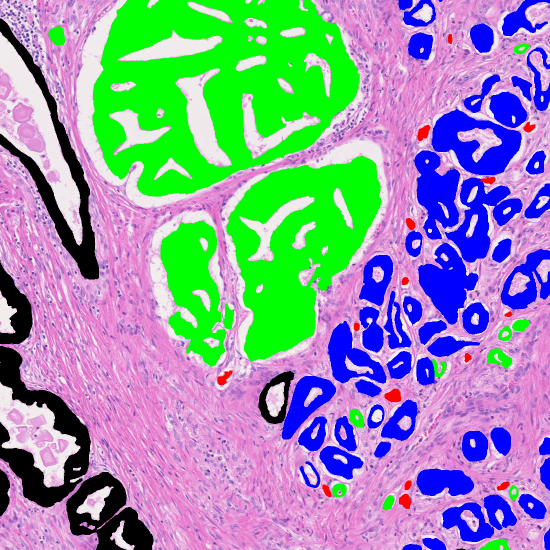
\includegraphics[width=0.9\columnwidth]{assets/ex_gt.png}
        \subcaption{Label image}
      \end{subfigure}

      \begin{subfigure}[t]{0.33\columnwidth}\centering
        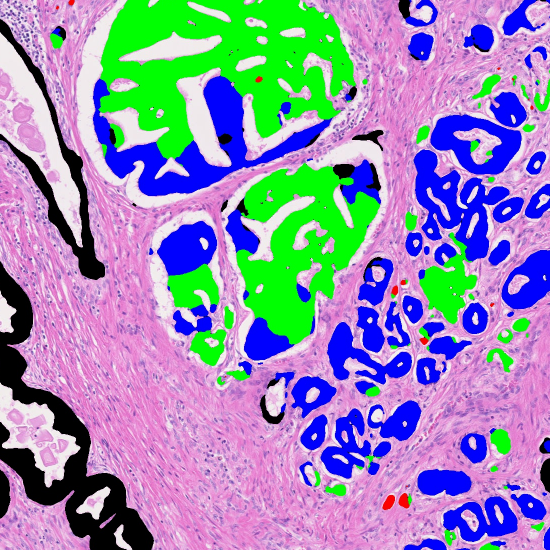
\includegraphics[width=0.9\columnwidth]{assets/ex_pr.png}
        \subcaption{Output image}
      \end{subfigure}
    \end{tabular}
    \label{fig:example}
    \caption{Example output of our U-Net model}
    \label{fig:dl_sample}
  \end{figure}
\end{frame}

\begin{frame}{Material and method}
  The IoU (Intersection over union) calculated by the Jaccard index of the U-Net model were 0.765 for the training datasets and 0.737 for the validation datasets.
  \begin{align}
    \label{eq:iou}
    Jaccard\,index = & \; \frac{|PR \cap GT|}{|PR \cup GT|} \\[5mm]
    PR: \mbox{Prediction} & \;\; GT: \mbox{Ground truth} \nonumber
  \end{align}
\end{frame}

\begin{frame}{Material and method}
  Now we developed the client/server applications (Fig.\ref{fig:arch}) for this study.
  \par
  \vspace{0.5zh}
  The client is installed into Raspberry Pi 4 Model B computer that is connected the microscopic camera via USB and designed to send microscopic image to server with trained U-Net DL model, and receive the semantic segmentation result, integrate the overlay images for the user pathologist.
  \begin{figure}\centering
    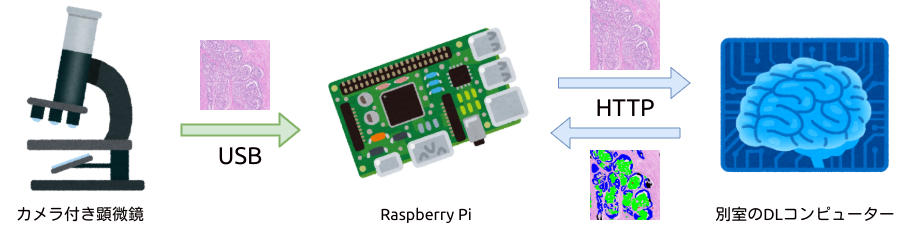
\includegraphics[width=0.8\columnwidth]{assets/arch.png}
    \caption{Architecture of the client and server applications}
    \label{fig:arch}
  \end{figure}
\end{frame}

\begin{frame}{Material and method}
  The DL system and the client/server applications were all written in Python and work on Linux-based computers. Especially the DL system uses PyTorch and the client uses GTK+/GStreamer. The source codes are all available on GitHub under 2-clause BSD license. \cite{gh-prostate}\cite{gh-pai}
\end{frame}

\begin{frame}{Result}
  Here's how it's actually used (Fig.\ref{fig:in_action}).
  \begin{figure}[t]\centering
    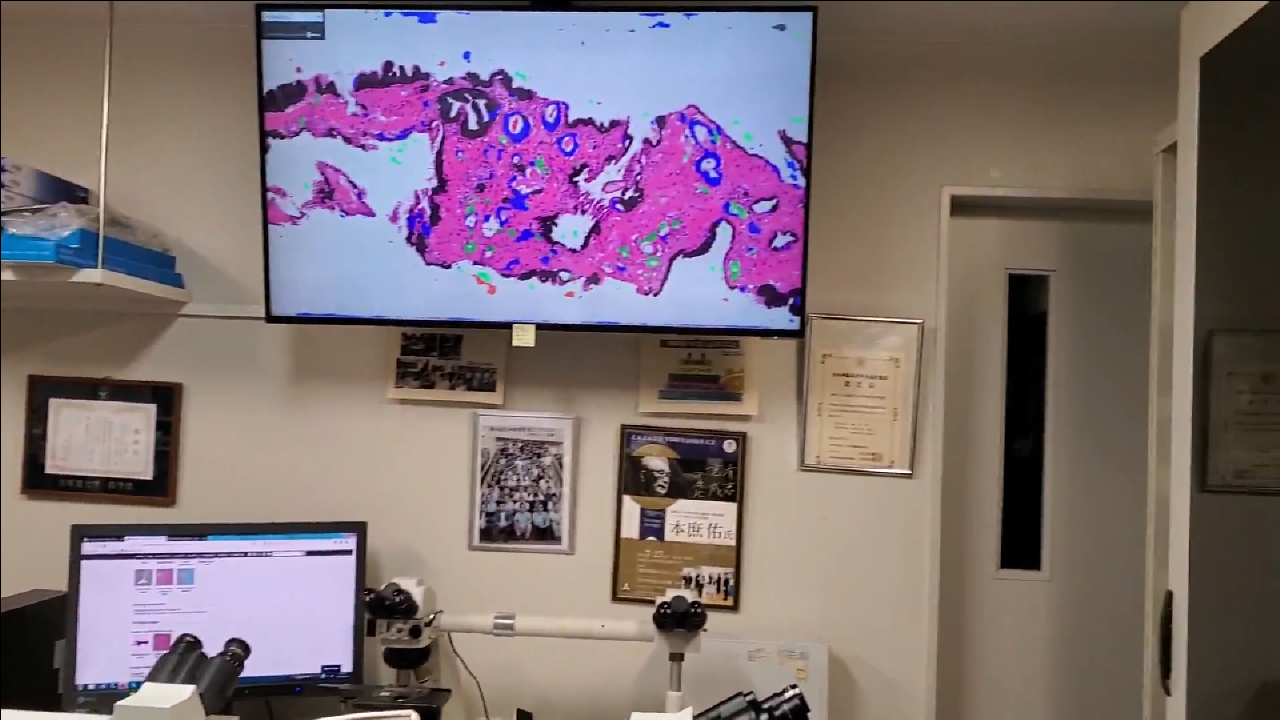
\includegraphics[width=\columnwidth, keepaspectratio]{assets/thumb.png}
    \caption{The client application in action (\href{https://drive.google.com/file/d/16hUGZ2jU2Def9N5ozNaZnLvjnWc-kkNP/view}{Link to the movie})}
    \label{fig:in_action}
  \end{figure}
\end{frame}

\begin{frame}{Result}
  Harnessing a computer with sufficient performance, we can get the results of DL analysis in as little as 20 seconds after clicking the analyze button on the screen. This means now any pathologists can try to use our DL model diagnosis without any effort or hassle of the non-integrated system.
  \par
  \vspace{0.5zh}
  However, it also means we have to wait for at least about 20 seconds; 10 seconds to analyze one Full HD 1920×1080 image still by the computer with dual nVIDIA GeForce GTX 1080 Ti, additional a few seconds to transfer the result image data.
\end{frame}

\begin{frame}{Result}
  We were faced with the throughput limit of the Raspberry Pi's calculation power. Simple preview monitoring of the USB-connected camera was exceeding the small computer's throughput, that resulted in frame dropping.
  \par
  \vspace{0.5zh}
  And there was also a delay to alpha composite the result image on the original one. The poor throughput hinders user experience of the client software.
\end{frame}

\begin{frame}{Discussion}
  We found user pathologists were grateful for the function just to save the image of the microscopic view without any analytics. Up until now, microscopic camera was connected to display directyl via HDMI. With the Raspberry Pi in between the camera and the display, we can now take photograph and analyze in addition to usage so far. \par
  \vspace{0.5zh}
  Users experienced as if the microscope camera was augmented in functional extension of itself.
\end{frame}

\begin{frame}{Conclusion}
  We discoverd the new side of Raspberry Pi as an add-on for the microscope camera. Though it is low cost as 7,000 yen, the throughput was not sufficient to handle Full HD images. \par
  \vspace{0.5zh}
  Future improvement may let us enable handling HD movie DL diagnosis.
\end{frame}

\begin{frame}{References}
  \begin{figure}
    \beamertemplatetextbibitems
    \bibliographystyle{junsrt}
    \bibliography{refs}
  \end{figure}
\end{frame}

\end{document}
